%%% Ch.3: Methodology %%%
\chapter{Methods} \label{ch:method}



\section{Markov chain Monte Carlo methods}
 One common way to effectively simulate systems with a large number of degrees of freedom is to apply Monte-Carlo simulations \cite{newman1999monte}. 
 
 We apply the Metropolis Monte Carlo method based on Markov chain. The main idea is to construct a Markov chain which has the given probability distribution \eqref{partitionfunction} as its equilibrium distribution . In Markov chain Monte Carlo methods (often referred to as MCMC methods),  the next sample is dependent on the last accepted one.  
 
  \par We use the Metropolis algorithm  \cite{doi:10.1063/1.1699114}. For generating an appropriate random set of states according to the given probability distribution \eqref{partitionfunction}, the conditions of ergodicity and detailed balance should be placed on the Markov chain.  
  Ergodicity means that algorithm can generate any state $u_{new}$ from any other state $u_0 $ in a finite number of steps. In physics the detailed balance means that each elementary process is in equilibrium with its reverse process. Detailed balance condition can be written as follows:
  \begin{equation}
  \label{detailedbalance}
  p_{u_0} P(u_0 \rightarrow u_{new} ) = p_{u_{new}} P( u_{new} \rightarrow u_0),
  \end{equation}
  where $P(u_0\rightarrow u_{new} )$ is the transition probability from state $u_0$ to $u_{new}$. Here, $p_{u_0},p_{u_{new}}$ are stationary Gibbs distribution probabilities: $p_{u_0} = e ^{-H(u_0)}/Z $.   Following a common way, we introduce the acceptance ratio $A(u_0 \rightarrow u_{new})$ and write:
  \begin{equation*}
  P(u_0 \rightarrow u_{new}) = g(u_0 \rightarrow u_{new}) A(u_0 \rightarrow u_{new}),
  \end{equation*}
where $g(u_0  \rightarrow u_{new} )$ is the selection probability that algorithm will generate a state $u_{new}$ from an initial state $u_0$. 

\subsection{Monte Carlo for self-avoiding walks}
 The self-avoiding walks model was studied before by several methods. The methods to generate states could be divided into two groups, referring to fixed-length ensembles and variable-length ensembles. 
 
One of the trivial methods for sampling chains of fixed length slithering-snake, or BEE reptation, move \cite{Caracciolo2011}.  The idea is to delete a node from one end of the walk and add a new node at the other end of conformation. We implement this update for XY model and discuss in Section \ref{sec:snake}. 

One of the variable-length algorithms is the Beretti-Sokal method \cite{Berretti1985}. The algorithm has two types of elementary updates: positive move and negative move. The positive step is implemented by appending an edge to the endpoint of the conformation. The negative update is deleting the last edge. The algorithm is easy to implement and allows to study properties of self-avoiding ensembles and extract general properties,  such as critical exponent $\nu$ from \eqref{r_scale}. However, these method is inefficient for studying region of structural phase transition in  interacting self-avoiding walks \cite{Nidras_1996} and the simplest heteropolymer \cite{Faizullina2021}. Efficient degradation stems from the form partition function for grandcanonical assemble.  

The other is well-know and widely used methods is growth algorithms. The review of growth algorithms is made thanks to Prelberg's material \cite{prelberg}. 

 The most trivial way to generate SAWs is to use Simple sampling. The algorithm starts from the origin point and each step attempts draw one of the neighbouring sites chosen randomly using uniform distribution. If the site is occupied, the algorithm rejects walk and starts again from the beginning. This method is easy to implement and its samples are uniform and independent. But the method is inefficient due to a large number of rejections caused by collision.

One  more sophisticated growth method is Rosenbluth Sampling. This method based on the steps when algorithm attempts to draw one of the unoccupied neighbouring sites chosen randomly and uniformly from the origin points and aims to generate the SAW of the chosen $N$. If there is none of non-visiting sites, the algorithm rejects entire walk and start again. The visiting only  unoccupied neighbouring leads to increasing performance. However, the number of wasted attempts is still large. Grassberger introduced Pruned and Enriched Rosenbluth Method (PERM) with a vie to improve sampling \cite{PhysRevE.56.3682}. Its modification is controlling the weights of SAWs copying (enrichment) states with large weights and occasional removing (pruning) conformations with low weights. 

One of improved versions  of PERM is flat histogram PERM (flatPERM) based on the fact that number of samples generated by PERM algorithm for each $N$ is roughly constant. The method generates flat histogram algorithm in system size and allows to calculate the coefficients of the series expansion in terms of the dependent variables on $J$. This method was applied to simulate Ising model on SAWs \cite{PhysRevE.104.024122}. FlatPERM is an efficient Monte Carlo method which allows to get functions of $J$ and avoid analyzing of the separate points. However, the method gets slower for large $N$.

We choose to implement snake-like, or BEE reptation, move to generate structural states with the aim to simulate large $N$ which would be quite difficult in practice using sophisticated FlatPERM. In order to improve sampling of SAWs, we also implement other update. In the Section \ref{sec:myalgorithm}, we discuss implement method applied to study XY model on SAWs. 


\section{MCMC of three updates} \label{sec:myalgorithm}
In this work, we construct the Markov Chain Monte Carlo method for fixed-length chain consisting of three types of updates. We refer to them as Snake-like step, Reconnection and Wolff Cluster update. In each iteration, the algorithm chooses the update according to set of probabilities. We define these probabilities as $P_{local}$,$P_{reconnect}$ and $P_{Wolff}$ respectively. The sum of probabilities is always equal to one: $P_{local} + P_{reconnect} + P_{Wolff} = 1$. This algorithm was described and used to study Ising model on SAWs \cite{PhysRevE.104.054501}. 


  \begin{figure}
	\centering
	%\captionsetup{justification=centering}
	\begin{subfigure}[b]{0.45\textwidth}
		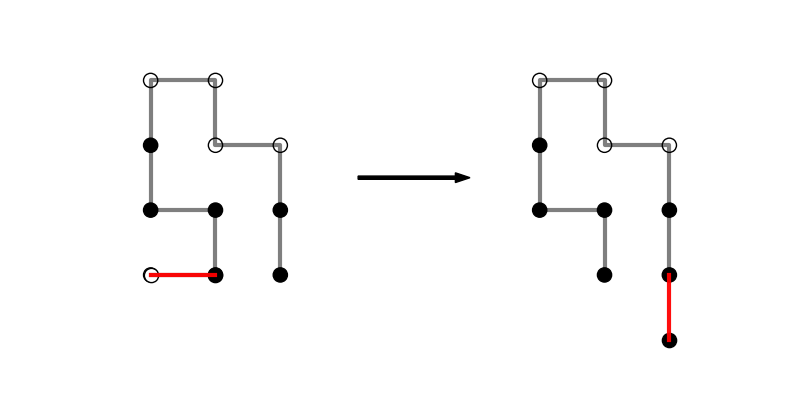
\includegraphics[width=\textwidth]{Images/snakeupdate.png}
		\caption{ Example of snake update. } 
		\label{fig:snake}
	\end{subfigure}
	\begin{subfigure}[b]{0.45\textwidth}
		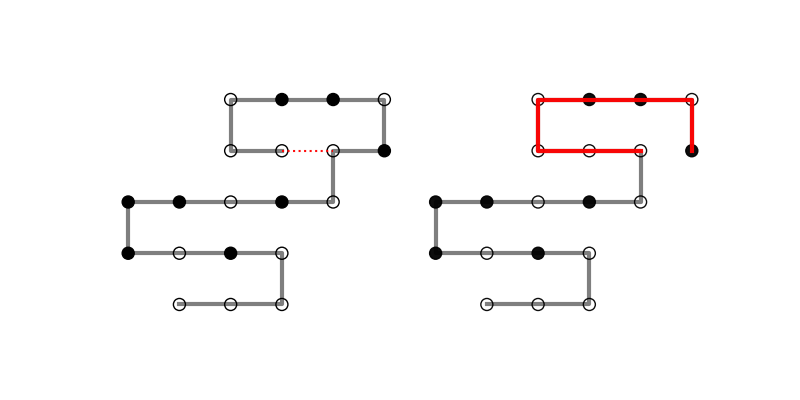
\includegraphics[width=\textwidth]{Images/reconnect.png}
		\caption{  Example of reconnect update. }
		\label{fig:reconnect}
	\end{subfigure}
	\caption{ Examples for both algorithm moves: snake-like and reconnect. These updates allow to generate conformations.   }
	\label{fig:UpdateSaw}
\end{figure}
 
\subsection{Snake-like algorithm} \label{sec:snake}
This is classical method to generate SAWs which brings to mind snakes move  \cite{Binder2010}. The snake move is a bilocal reptation update. The algorithm removes a monomer from one end and adds a monomer to the other end as it is illustrated in Figure \ref{fig:snake}. Spin angle value $\theta_{new}$ and the direction in conformation are randomly generated. The direction is chosen uniformly with the probability $\frac{1}{2d}$, where $d$ is the dimensions of the lattice. The spin angle variable $\theta_{new}$ is generated uniformly $\theta_{new} \sim U(-\pi, \pi)$. The new generated state is simply accepted  according to the Metropolis rule:
\begin{equation}
\label{accratios}
A(u_0  \rightarrow u_{new} ) =  
\begin{cases}
e^{-J(E_{u_{new}}-E_{u_0})}, & \text{if $E_{u_{new}}-E_{u_0}>0$;}\\
1, & \text{otherwise}.
\end{cases}
\end{equation}

The snake update is very convenient to implement and the time and the  memory complexity $O(1)$. However, the autocorrelation time is quite long for magnetic variables and for structure  $ \eta \sim N^2 $ and the system can be locked in the frozen states when both ends of the conformation are surrounded by $2d$ neighbors. To overcome the problem, we also use Reconnect update to accelerate conformations generation and Wolff-cluster algorithm to effectively explore spin configuration space. 


\subsection{Reconnect}


Reconnect is a non-local update based on ideas of Worm algorithm for Ising model \ref{fig:reconnect} \cite{Worm}.   In this system update, only connections of conformation are changed. The acceptance probability is always equal to one as the energy does not change. 

The algorithm allows system to return from frozen stated. The reconnect algorithm also allows to effectively generate conformations. The time complexity $O(N)$.  

\subsection{Wolff cluster update}
% https://math.stackexchange.com/questions/13261/how-to-get-a-reflection-vector
This is classical The Wolff algorithm for Monte Carlo simulation which we use to improve sampling of the spin configuration space  \cite{wolff}. 

The main idea of the update is to form the cluster $C$ of spins and flip its spins. The update rules should obey the detailed balance condition. We follow the classical way of cluster update implementation for XY model discussed in Ref. \cite{newman1999monte}. 

  \begin{figure}
	\centering
	\captionsetup{justification=centering}
	\begin{subfigure}[b]{0.45\textwidth}
		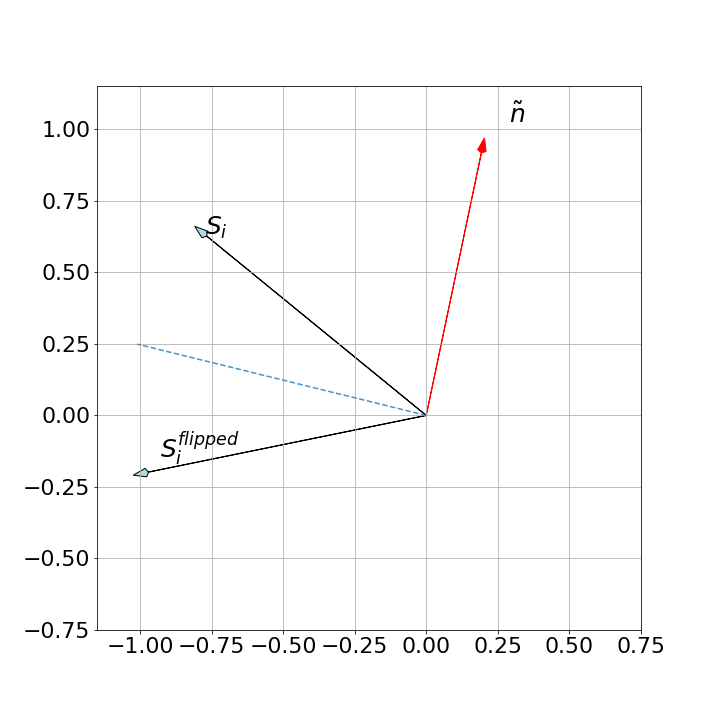
\includegraphics[width=\textwidth]{Images/cluster_flip.png}
		\caption{ Example of spin flip. The solid red arrow is randomly chosen unit vector $\vec{n}$. The dashed blue line is perpendicular plane  }
		\label{fig:clusterflip}
	\end{subfigure}
	\begin{subfigure}[b]{0.45\textwidth}
		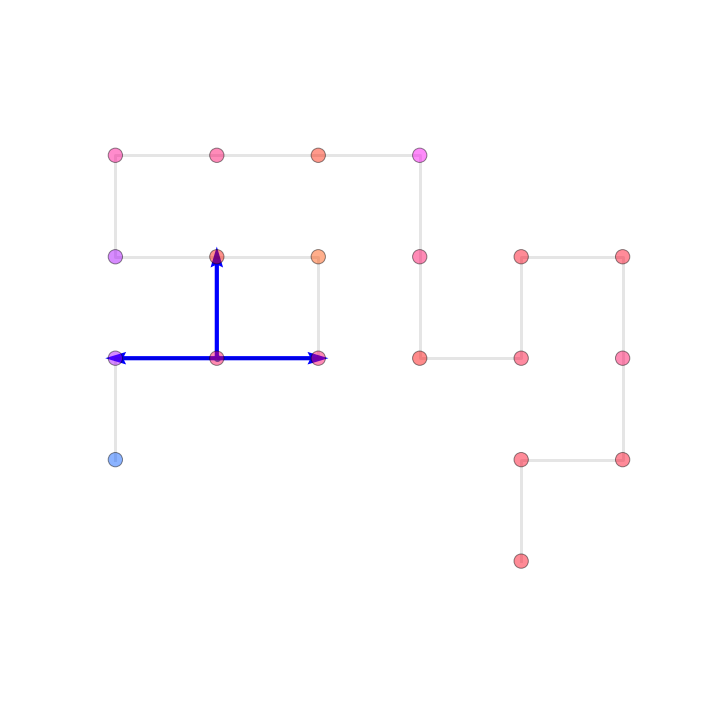
\includegraphics[width=\textwidth]{Images/state_example_cluster.png}
		\caption{  Example of cluster grow from the starting point. Blue arrows shows directions to attempt to add new spins to cluster. The color of nodes represents spins values. }
		\label{fig:clustergrowth}
	\end{subfigure}
	\caption{ Cluster Update for XY on SAWs.  }
	\label{fig:ClusterUpdate}
\end{figure}


To flip spin  using chosen direction $\vec{n}$ means to change sign of vector $ \vec{n} \vec{S_i} (\theta_i) = \vec{n}(\cos \theta_i \sin \theta_i  )$  to the opposite, see Figure \ref{fig:clusterflip}. 
 
 


\begin{enumerate}
	
	\item Choose randomly the spin $\overrightarrow{S_{start}}$ from the chain using discrete uniform distribution. 
	
	\item Choose the direction on the unit circle $\overrightarrow{n}$ using uniform distribution $ \theta_{new} = U(-\pi, \pi)$: $\overrightarrow{n} = [\cos(\theta_{new}), \sin(\theta_{new})]$.
	
	\item Update the chosen monomer $\overrightarrow{S_{start}}$. To do it, we need to change sign of $ \vec{n}  \overrightarrow{S_{start}} $ to the opposite. This action is the subtraction the reflected  $\vec{n}$  from $ \overrightarrow{S_{start}} $. Therefore, the flip is implemented as following: $\overrightarrow{S_{start}} := \overrightarrow{S_{start}} - 2 \times ( \overrightarrow{S_{start}} \vec{n}) \times \vec{n}$. We add this flipped spin to the cluster $C$ and point it as flipped.
	
	\item Take one spin $ \overrightarrow{S_{i}}$ from the cluster to visit all its neighbors $S_j$, see Figure \ref{fig:clustergrowth}. Add new spin to the cluster with the probabilities $P_{add}(\overrightarrow{S_{i}}, \overrightarrow{S_{j}} ) = 1 - \exp \left(2J (\overrightarrow{S_{i}}\overrightarrow{n})( \overrightarrow{S_{j}} \overrightarrow{n} ) \right)$, where $\overrightarrow{S_{i}}\overrightarrow{n}$ is a dot product. 
	
	If the spin $\overrightarrow{S_{j}}$ was added to cluster and has not been flipped, make update: $\overrightarrow{S_{j}} : = \overrightarrow{S_{j}} - 2 \times ( \overrightarrow{S_{j}} \vec{n}) \times \vec{n}$. Point the spins as flipped.
	
	After visiting all neighbors, remove  $ \overrightarrow{S_{i}}$ from the cluster.
	
	\item Repeat the previous step until cluster is empty. 
	
\end{enumerate}

The algorithm effectively sample spin configurations and keep the conformation fixed. The time complexity $O(N)$. 
 


